\documentclass[oneside]{ctexbook}
\usepackage{ctex}
\usepackage[utf8]{inputenc}
\usepackage{amsmath}
%\usepackage{amsthm}
\usepackage{ntheorem}
\usepackage{booktabs}
\usepackage{caption}
\usepackage{listings}
\usepackage[dvipsnames]{xcolor}
\usepackage{xeCJK}
\usepackage{bm}
\usepackage{fancyhdr}
\usepackage{graphicx}
\usepackage{amssymb}
\usepackage{mathrsfs}
\usepackage{titlesec, blindtext, color}
\usepackage{arydshln}
\usepackage{hyperref} 
\usepackage[OT1]{fontenc}
\usepackage{geometry}
\usepackage{comment}
\usepackage{extarrows}
\usepackage{inconsolata}
\usepackage{enumitem}


\geometry{a4paper,scale=0.8}

\hypersetup{hidelinks,
	colorlinks=true,
	allcolors=black,
	pdfstartview=Fit,
	breaklinks=true
}

\ctexset{
	 chapter = {
		name = {第,部分},
		format = \linespread{1.0}\zihao{1}\bfseries\sffamily\centering,
		nameformat = {\fontsize{30pt}{0pt}\centering\vspace{15pt}},
		titleformat = {\centering},
		number = \chinese{chapter},
		numberformat = \sffamily,
		aftername = {},
		beforeskip = {7pt},
		afterskip = {18pt},
		aftername = {\\},
		pagestyle = plain,
	},
	section={
		%format用于设置章节标题全局格式,作用域为标题和编号
		%字号为小三,字体为黑体,左对齐
		%+号表示在原有格式下附加格式命令
		format+ = \zihao{-1} \heiti \raggedright\centering,
		%name用于设置章节编号前后的词语
		%前、后词语用英文状态下,分开
		%如果没有前或后词语可以不填
		name = {,.\,},
		%number用于设置章节编号数字输出格式
		%\chinese输出section编号为中文,\arabic输出为阿拉伯数字
		number = \Roman{section},
		%beforeskip用于设置章节标题前的垂直间距
		%ex为当前字号下字母x的高度
		%基础高度为1.0ex,可以伸展到1.2ex,也可以收缩到0.8ex
		beforeskip = 1.0ex plus 0.2ex minus .2ex,
		%afterskip用于设置章节标题后的垂直间距
		afterskip = 1.0ex plus 0.2ex minus .2ex,
		%aftername用于控制编号和标题之间的格式
		%\hspace用于增加水平间距
		aftername = \hspace{0pt}
	},
	subsection={
		format+ = \zihao{-2} \kaishu  \raggedright,
		%仅输出subsection编号且为中文
		number = \roman{subsection},
		name = {,.},
		beforeskip = 1.0ex plus 0.2ex minus .2ex,
		afterskip = 1.0ex plus 0.2ex minus .2ex,
		aftername = \hspace{0pt}
	},
	subsubsection={
		%设置对齐方式为居中对齐
		format+ = \zihao{-3} \fangsong,
		%仅输出subsubsection编号,格式为阿拉伯数字,打字机字体
		number = \ttfamily\arabic{subsubsection},
		name = {,.},
		%beforeskip = 1.0ex plus 0.2ex minus .2ex,
		afterskip = 1.0ex plus 0.2ex minus .2ex,
		aftername = \hspace{0pt}
	}
}

\fancyhf{}
\fancyhead[L]{
	\begin{minipage}[c]{0.06\textwidth}
		\hyperlink{Index}{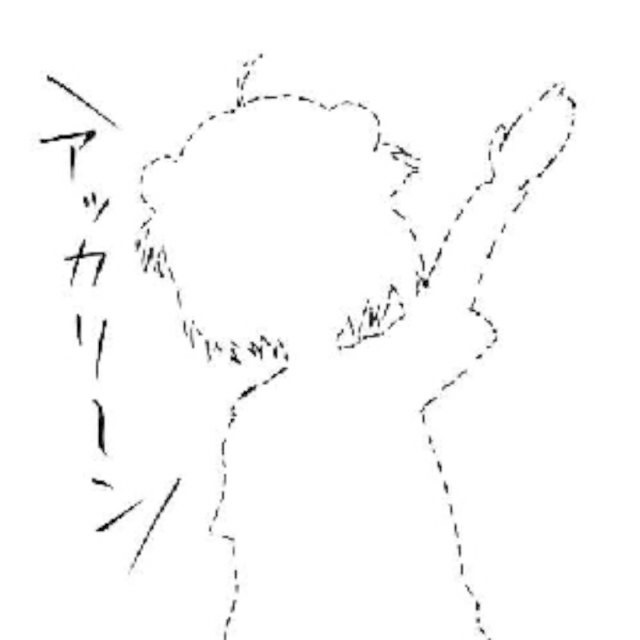
\includegraphics[height=7.5mm]{1.jpg}}
	\end{minipage}
	\begin{minipage}[c]{0.4\textwidth}
		\hyperlink{Index}{赛博题本}
	\end{minipage}}
\fancyhead[R]{
    \begin{minipage}[r]{0.1\textwidth}
	\href{https://qifengggg.github.io/}{奇峰}
    \end{minipage}
}
\cfoot{\thepage}

\pagestyle{fancy}
%\renewcommand{\qedsymbol}{$\blacksquare$}

\renewcommand{\labelenumi}{\rm (\Alph{enumi})}
\renewcommand{\labelitemi}{$ \square $ }
\newcommand\dis{\displaystyle}
\newcommand\dsqrt{\displaystyle\sqrt}
\newcommand{\pprime}{{\prime\prime}}
\newcommand{\red}{\textcolor{red}}
\newcommand{\sssubsection}[1]{\noindent\textbf{#1}}

\title{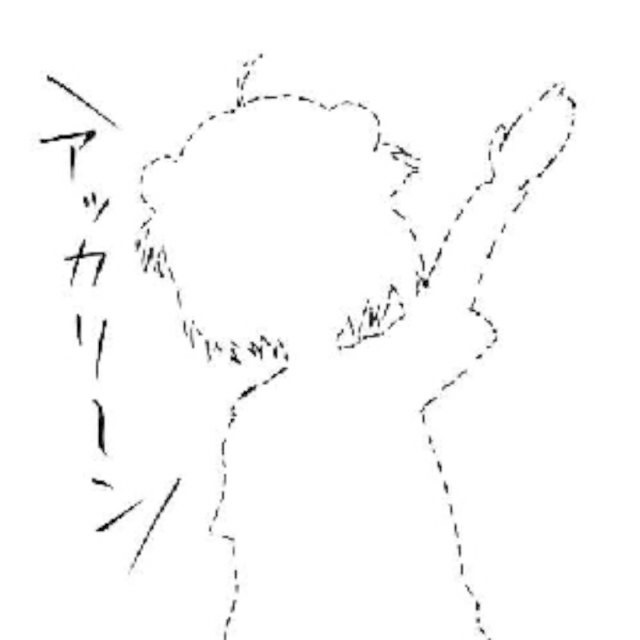
\includegraphics[scale=0.6]{1.jpg}\\ \textsf{赛博题本}}
\author{奇峰}
\date{之前}

\begin{comment}
	\newtheorem{def1}{定义}[chapter]
	\newtheorem{theo1}{定理}[chapter]
	\newtheorem{func1}{方法}[chapter]
	\newenvironment{proof}[1][证明]{\noindent\newline\textbf{#1}\quad{}}{\hfill $\blacksquare$\par}
	%\newenvironment{<环境名称>}[<参数个数>][<首参数默认值>]{<环境前定义>}
	%							{<环境后定义>}
	
	
	\newenvironment{Def}[1][\quad{}]{\begin{def1}\textbf{#1}}{\end{def1}}
	\newenvironment{Theo}[1][\quad{}]{\begin{theo1}\textbf{#1}}{\end{theo1}}
	\newenvironment{Func}[1][\quad{}]{\begin{func1}\textbf{#1}}{\end{func1}}
	\end{comment}

\begin{document}

\allowdisplaybreaks[4]

\theoremseparator{}
\newenvironment{Field}[1][\quad{}]{\noindent\newline\textbf{#1}\hfill}{}

\newcounter{cntQ}
\newcounter{cntA}
%\newtheorem{quest}{问题}
\newenvironment{Quest}[1][\quad{}]
{\begin{Field}\textbf{\stepcounter{cntQ}问题\thecntQ\quad{}{\rm #1}}\vspace{5pt}\noindent\newline}{\end{Field}}

%\newtheorem{answer}{答案}
\newenvironment{Answer}[1][\quad{}]
{\begin{Field}\textbf{\stepcounter{cntA}答案\thecntA\quad{}{#1}}\vspace{5pt}\noindent\newline}{\end{Field}}

\newenvironment{BulletItemize}
{\renewcommand{\labelitemi}{\textbullet}\begin{itemize}[topsep = 0pt]
}{\end{itemize}}

\setlength{\parindent}{0pt}
\setlength{\parskip}{5pt}

\newcommand{\from}[1]{\hypertarget{#1}{}}
\newcommand{\goto}[1]{\quad{}\hyperlink{#1}{$ \diamondsuit $ }\hypertarget{K#1}{}}
%\newcommand{\getback}[1]{\begin{flushright}\hyperlink{K#1}{$ \blacksquare $ }\end{flushright}}

\newcommand{\getback}[1]{\quad{}\hyperlink{K#1}{$ \blacksquare $ }}
\newcommand{\qline}{\underline{~~~~~~~~}}

\newenvironment{quest}[1][\quad{}]
{\begin{Field}\textbf{
	\stepcounter{cntQ}问题\thecntQ\quad{}{\rm #1}}\goto{#1}\vspace{5pt}\noindent\newline}{\end{Field}}

\newenvironment{answer}[2][\quad{}]
{\from{#1}\begin{Field}\textbf{
	\stepcounter{cntA}答案\thecntA\quad{}{#2}}\vspace{5pt}\getback{#1}}{\end{Field}}

\frontmatter
\maketitle

\hypertarget{Index}{}
\tableofcontents

\mainmatter

\chapter{错题}
\section{练习}

\begin{Quest}[\goto{E1}]
    $\dis {\displaystyle\lim_{n\rightarrow \infty}}\sin\sqrt{4n^2+n}\pi=() $
    \begin{enumerate}
        \item $ 0 $ 
        \item $ 1 $ 
        \item $ \dis \frac{\sqrt 2}{2} $ 
        \item 不存在
    \end{enumerate}
\end{Quest}

\begin{quest}[660T9]
    $$
        I = {\displaystyle\lim_{x\rightarrow 0}}\dfrac{\dis \int_{x^2}^x\dfrac{\sin xt}{t}\mathrm{d}t}{x^2}
        =\qline.
    $$ 
\end{quest}

\begin{quest}[660T11]
    设 $ a>0 $ ,则$$
        {\displaystyle\lim_{x\rightarrow 0^+}}(x^2+x)^{x^a} = \qline.
    $$ 
\end{quest}

\begin{quest}[660T17]
    设 $ a,b $ 为常数,且 $ \dis {\displaystyle\lim_{x\rightarrow \infty}}(\dsqrt[3]{1-x^6}-ax^2-b) = 0 $ ,
    则 a=\qline,b=\qline.
\end{quest}

\begin{quest}[660T21]
    已知 $ x\rightarrow0 $ 时 $ \dis F(x) = \int_0^{x-\sin x}\ln(1+t)\mathrm{d}t $ 是 $ x^n $ 的同阶无穷小,
    则 $ n = \qline. $ 
\end{quest}

\begin{quest}[660T27]
    设$ \dis f(x) = \begin{cases}
        \dfrac{\ln (1+bx)}{x},& x\neq0\\-1,& x = 0
    \end{cases} $ ,其中 $ b $ 为常数,$ f(x) $ 在定义域上处处可导,则 $ f'(x) = \qline. $ 
\end{quest}

\begin{quest}[660T28]
    设 $ f(x) = \begin{cases}
        x^2,&x\leq 0\\ 
        x^a\sin \dfrac{1}{x},& x > 0
    \end{cases} $ ,若 $ f(x) $ 可导,则 $ a $ 满足(),若 $ f'(x) $ 连续,则 $ a $ 满足\qline.
\end{quest}

\begin{quest}[660T29]
    设 $ f(x) $ 是以 $ 3 $ 为周期的可导函数且为偶函数,$ f'(-2) = -1 $ ,则
    $ {\displaystyle\lim_{h\rightarrow 0}}\dfrac{h}{f(5-2\sin h) - f(5)} = \qline. $ 
\end{quest}

\begin{quest}[660T30]
    设 $ f(x) $ 在 $ x= 0 $ 可导且 $ f(0) = 1,f'(0)=3 $ ,则数列极限
    $$
    \dis I = {\displaystyle\lim_{n\rightarrow \infty}}
    (f(\dfrac{1}{n}))^{\dfrac{\frac{1}{n}}{1-\cos\frac{1}{n}}} =\qline.
    $$
\end{quest}

\begin{quest}[660T33]
    $ f(x) = x^2(x+1)^2(x+2)^2(x+3)^2 $,则 $ f^"(0) =$\qline. 
\end{quest}

\begin{quest}[660T34]
    设 $ y = y(x) $ 由参数方程 
    $ \begin{cases}
        x = \dfrac{1}{2}\ln (1+t^2)\\ y = \arctan t
    \end{cases} $ 确定,则 $ \dfrac{\mathrm{d}y}{\mathrm{d}x} = (),
    \dfrac{\mathrm{d}^2y}{\mathrm{d}x^2}=(),y = y(x) $ 在任意点处的曲率 $ K $ 为\qline.
\end{quest}

\begin{quest}[660T38]
    设函数 $ y=f(x) $ 为由方程 $ \dis \int_b^y(2+\sin^2t)\mathrm{d}t = 1 $ 确认的
    隐函数,则 $ \mathrm{d}y =$\qline.
\end{quest}

\begin{quest}[660T40]
    设 $ f(x) =\ln \dfrac{1-2x}{1+3x} $ ,则 $ f^{(3)}(0) = $\qline. 
\end{quest}

\begin{quest}[660T48]
    曲线 $ y = \sqrt{4x^2+x}\ln (2+\dfrac{1}{x}) $ 的全部渐近线为\qline.
\end{quest}

\begin{quest}[660T49]
    设函数 $ f(x) $ 在 $ x = 0 $ 处连续,
    且 $ {\displaystyle\lim_{x\rightarrow 0}}\dfrac{f(x)}{e^x - 1} = 2 $,
    则曲线 $ y = f(x) $ 在 $ x = 0 $ 处的法线方程为\qline.
\end{quest}

\begin{quest}[660T51]
    设 $ \dis \int xf'(x)\mathrm{d}x = \arctan x + C $ ,则 $ f(x) = \qline. $ 
\end{quest}

\begin{quest}[660T52]
    $ \dis I = \int \dsqrt[]{\dfrac{3-2x}{3+2x}}\mathrm{d}x = \qline. $ 
\end{quest}

\begin{quest}[660T59]
    $ \dis I = \int_0^1 \arcsin x \cdot \arccos x \mathrm{d}x =\qline. $ 
\end{quest}

\begin{quest}[660T60]
    $ \dis \int_0^1\left[\sqrt{2x-x^2}-\sqrt{(1-x^2)^3}\right]\mathrm{d}x = \qline. $ 
\end{quest}

\begin{quest}[660T64]
    设 $ f(x) = \max \{1,x^2\} $ ,则 $ \dis \int_1^x f(t)\mathrm{d}t = \qline. $ 
\end{quest}

\begin{quest}[660T68]
    $ \dis I = \int_1^{+\infty} \dfrac{2x^2+bx+a}{x(2x+a)}-1\mathrm{d}x $ ,则 $ a = \qline,b = \qline. $ 
\end{quest}


\section{考试}
\begin{Quest}[C1T5\goto{T1}]
    设 $ a>0 $ ,则 $\dis {\displaystyle\lim_{n\rightarrow +\infty}}n^2(\sqrt[n]a-\sqrt[n+1]a)=() $

    \begin{enumerate}
        \item 不存在且非无穷大
        \item 0
        \item $ \ln a $ 
        \item $ \infty $ 
    \end{enumerate}
\end{Quest}

\begin{Quest}[C1T11\goto{T2}]
    已知 $ {\displaystyle\lim_{x\rightarrow +\infty}}\left(\dis\sqrt{x^2+x+1}-ax-b\right)=0 $ ,
    则 $ a+b=\qline. $ 
\end{Quest}

\begin{Quest}[C1T12\goto{T3}]
    设函数 $\dis f(x) = {\displaystyle\lim_{t\rightarrow x}}
    \left(\frac{\sin t}{\sin x}\right)^{\dis \frac{x}{\sin t-\sin x}} $ ,
    则 $ f(x) $ 的可去间断点为 $ x=\qline. $ 
\end{Quest}

\begin{Quest}[C1T15\goto{T4}]
    若 $ a>0,b>0 $ ,则 $ \dis {\displaystyle\lim_{n\rightarrow +\infty}}
    \left(\frac{\sqrt[n]a+\sqrt[n]b}{2}\right)^n = \qline. $ 
\end{Quest}

\begin{Quest}[C1T16\goto{T5}]
    $ \dis {\displaystyle\lim_{x\rightarrow \frac{\pi}{4}}}(\tan x)^{\dis\frac{1}{\cos x-\sin x}} = \qline. $ 
\end{Quest}

\begin{Quest}[C1T20\goto{T6}]
    设函数 $\dis f(x)=\ln x + \frac{1}{x} $.
    \begin{itemize}
        \item[$ \blacksquare $ ] 求 $ f(x) $ 最小值;
        \item[$ \square $ ] 设数列 $ \{x_n\} $ 满足 $ \dis \ln x_n + \frac{1}{x_{n+1}}<1 $ ,证明
        $ {\displaystyle\lim_{n\rightarrow \infty}}x_n $ 存在,并求该极限。
    \end{itemize}
\end{Quest}

\begin{Quest}[C1T22\goto{T7}]
    设函数 $ f(x) $ 满足 $a \leq f(x)\leq b,\ \forall x,y\in [a,b],|f(x)-f(y)|<|x-y|  $ .

    设 $ x_1\in[a,b] $ , $\dis x_{n+1}=\frac{1}{2}\left[x_n+f(x_n)\right] $ ,
    证明极限 $ {\displaystyle\lim_{n\rightarrow \infty}}x_n $ 存在,记为且满足
    $ c=f(c) $ .
\end{Quest}

\begin{quest}[C2T1]
    设 $ f(x) $ 具有二阶连续导数,
    且 $ f'(0) = 0,{\displaystyle\lim_{x\rightarrow 0}}\dfrac{f^"(x)}{|x|} = 1 $,
    则 ()
    \begin{enumerate}
        \item $ f(0) $ 是 $ f(x) $ 的极大值
        \item $ f(0) $ 是 $ f(x) $ 的极小值
        \item $ (0,f(0)) $ 是 $ f(x) $ 的拐点
        \item $ f(0) $ 不是 $ f(x) $ 的极值,$ (0,f(0)) $ 也不是曲线 $ y=f(x) $ 的拐点
    \end{enumerate} 
\end{quest}


\begin{quest}[C2T8]
    已知函数$$
    f(x) = \begin{cases}
        x,&x\leq 0\\
        \dfrac{1}{n},&\dfrac{1}{n+1}<x\leq \dfrac{1}{n}, n = 1,2,\dots
    \end{cases}
$$ 则()
\begin{enumerate}
    \item $ x=0 $ 是 $ f(x) $ 的第一类间断点
    \item $ x=0 $ 是 $ f(x) $ 的第二类间断点
    \item $ f(x) $ 在 $ x=0 $ 连续但不可导
    \item $ f(x) $ 在 $ x=0 $ 可导
\end{enumerate}
\end{quest}

\begin{quest}[C2T11]
    已知 $ y = y(x) $ 满足 $ y^3+x^3-3xy = 0 $ ,且存在斜渐近线,则该斜渐近线为\qline.
\end{quest}

\begin{quest}[C2T17]
    设 $ f(x) = \arctan \dfrac{1-x}{1+x} $ ,求高阶导数值 $ f^{(2020)}(0) $ 与 $ f^{(2021)}(0) $ 。
\end{quest}

\begin{quest}[C2T20]
    设 $ a $ 为常数,讨论方程 $ x^2=ae^x $ 的实根个数及其所在范围。
\end{quest}


\begin{quest}[C2T21]
    设函数 $ f(x) $ 在 $ [0,1] $ 连续, $ (0,1) $ 可导, $ c\in (0,1) $ , $ f(0)\neq F(1) $ ,
    则存在 $ \xi\in (0,1) $ , $ \eta\in (0,1) $ 使得 $$
        2\eta f(1) + (c^2-1)f'(\eta) = f(\xi)
    $$ 
\end{quest}

\begin{quest}[C2T22]
    设函数 $ f(x) $ 和 $ g(x) $ 在 $ [a,b] $ 上存在二阶导数,且 $ g^"(x)\neq 0, f(a)=f(b)=g(a)=g(b) = 0 $ ,
    则\begin{itemize}
        \item[$ \blacksquare $ ] 在开区间 $ (a,b) $ 内 $ g(x)\neq 0 $ 
        \item 在开区间 $ (a,b) $ 内至少存在一点 $ \xi $ ,使得$$
            \dfrac{f(\xi)}{g(\xi)} = \dfrac{f^"(\xi)}{g^"(\xi)}
        $$ 
    \end{itemize}
\end{quest}


\newpage
\chapter{答案及注意事项}
\section{练习}

%\hypertarget{T1}{}
\from{E1}
\begin{Answer}[求$ n $ 时,求出一个定值\getback{E1}]
    \begin{equation*}
        \begin{aligned}
            \dis {\displaystyle\lim_{n\rightarrow \infty}}\sin\sqrt{4n^2+n}\pi &=
            {\displaystyle\lim_{n\rightarrow \infty}}\sin(2n+\sqrt{4n^2+n}-2n)\pi \\
            &= {\displaystyle\lim_{n\rightarrow \infty}}\sin(\sqrt{4n^2+n}-2n)\pi \\
            &= {\displaystyle\lim_{n\rightarrow \infty}}\sin\dis\frac{n}{\dis\sqrt{4n^2+n}+2n}\pi \\
            &= \sin \frac{\pi}{4} = \frac{\sqrt 2}{2}
        \end{aligned}
    \end{equation*}
\end{Answer}

\begin{answer}[660T9]{通过换元法将 $ x $ 剔除出积分式}
    令 $ s = xt $ ,则有
    \begin{equation*}
        \begin{aligned}
            I&={\displaystyle\lim_{x\rightarrow 0}}
            \dfrac{\dis \int_{x^3}^{x^2}\dfrac{\sin s}{s}\mathrm{d}s}{x^2}\\&=
            {\displaystyle\lim_{x\rightarrow 0}} \dfrac{\dis \dfrac{\sin x^2}{x^2}\cdot 2x - 
            \dfrac{\sin x^3}{x^3}\cdot 3x^2}{2x} \\&= {\displaystyle\lim_{x\rightarrow 0}}
            \dfrac{2\sin x^2 - 3\sin x^3}{2x^2} = 1
        \end{aligned}
    \end{equation*}
\end{answer}

\begin{answer}[660T11]{不要先想象分类讨论的结果再补画靶子}
    令原极限 $ = I $ ,$ t = \dfrac{1}{x} $ ,则有
    \begin{equation*}
        \begin{aligned}
            I &= \exp\left\{{\displaystyle\lim_{t\rightarrow +\infty}}\dfrac{\ln \dfrac{t+1}{t^2}}{t^a}\right\}\\&=
            \exp\left\{{\displaystyle\lim_{t\rightarrow +\infty}}\dfrac{\ln(t+1)-2\ln t}{t^a}\right\}\\&=
            \exp\left\{{\displaystyle\lim_{t\rightarrow +\infty}}\dfrac{\dfrac{1}{t+1}-\dfrac{2}{t}}{at^{a-1}}\right\}
            \\&= \exp\left\{{\displaystyle\lim_{t\rightarrow +\infty}}\dfrac{-t-2}{a(t+1)t^{a+1}}\right\}\\&=
            \exp\left\{{\displaystyle\lim_{t\rightarrow +\infty}}\dfrac{-1}{a(a+1)t^{a+1}+a^2t^a}\right\} = 1
        \end{aligned}
    \end{equation*}
\end{answer}

\begin{answer}[660T17]{对根式,令 $ t=-\dfrac{1}{x^6}, x\rightarrow \infty  $,然后泰勒展开 }
    由于
    \begin{equation*}
        \begin{aligned}
            \dsqrt[3]{1-x^6} &= -x^2\dsqrt[3]{1-\dfrac{1}{x^6}} \\&\xlongequal{t = -\dfrac{1}{x^6}}
            -x^2\left(1+\dfrac{1}{3}t+o(t)\right) = -x^2\left(1-\dfrac{1}{3x^6}+o(x^{-6})\right)
        \end{aligned}
    \end{equation*}
    代回原极限,发现当且仅当 $ a = -1,b = 0 $ 时原极限成立。
\end{answer}

\begin{answer}[660T21]{利用一次洛必达法则后不要忘记分母的次数为 $ n-1 $ }
    由题,\begin{equation*}
        \begin{aligned}
            {\displaystyle\lim_{x\rightarrow 0}}\dfrac{F(x)}{x^n}&=
            {\displaystyle\lim_{x\rightarrow 0}}\dfrac{\dis \int_0^{x-\sin x}\ln(1+t)\mathrm{d}t}{x^n}\\&=
            {\displaystyle\lim_{x\rightarrow 0}}\dfrac{ln(1+x-\sin x)(1-\cos x)}{nx^{n-1}}\\&=
            {\displaystyle\lim_{x\rightarrow 0}}\dfrac{\frac{1}{6}x^3\cdot\frac{1}{2}x^2 }{nx^{n-1}} = a
        \end{aligned}
    \end{equation*}
    其中 $ a $ 是常数,故 $ n-1 = 5 $ ,即 $ n = 6 $ 。
\end{answer}

\begin{answer}[660T27]{注意题目要求的是单点还是函数}
    由 $ f(x) $ 在定义域的可导性,有 $ f(x) $ 在 $ x=0 $ 处可导,因此有 $ {\displaystyle\lim_{x\rightarrow 0}}f(x) = -1 $ ,
    故 $ b = -1 $ 。当 $ x \not=0 $ 时,可以直接得出 $ f'(x) = \dfrac{x-(x-1)\ln(1-x)}{(x-1)x^2} $ ;
    $ x=0 $ 时,由定义,\begin{equation*}
        \begin{aligned}
            f'(0) &= {\displaystyle\lim_{x\rightarrow 0}}\dfrac{f(x) - f(0)}{x - 0} \\&=
            {\displaystyle\lim_{x\rightarrow 0}}\dfrac{\dfrac{ln(1-x)}{x} + 1}{x} = -\dfrac{1}{2}
        \end{aligned}
    \end{equation*}
    故可以知道,
    $$
        f'(x) = \begin{cases}
            \dfrac{x-(x-1)\ln(1-x)}{(x-1)x^2},& x < 1, x \neq 0\\ 
            -\dfrac{1}{2},& x = 0
        \end{cases}
    $$ 
\end{answer}


\begin{answer}[660T28]{在写作业的时候不要听狗叫}
    $ f(x) $ 在 $ R \backslash \{0\} $ 上的可导性显然。而 \begin{equation*}
        \begin{aligned}
            f'_+(0) &= {\displaystyle\lim_{x\rightarrow 0^+}}\dfrac{f(x) - f(0)}{x - 0} \\&=
            {\displaystyle\lim_{x\rightarrow 0^+}}\dfrac{x^a\sin \frac{1}{x}}{x} = {\displaystyle\lim_{x\rightarrow 0^+}}
            x^{a-1}\sin \dfrac{1}{x}
        \end{aligned}
    \end{equation*}
    而 $ f'(x)_- = 0 $ ,当 $ f(x) $ 在 $ x = 0 $ 可导时,显然 $ a > 1 $ 。

    $ f'(x) $ 在 $ R\backslash \{0\} $ 上的连续性显然,而 $ f'(0) = 0 $ ,当 $ f'(x) $ 在 $ x = 0 $ 连续时,有 \begin{equation*}
        \begin{aligned}
            {\displaystyle\lim_{x\rightarrow 0}}f'(x) - f'(0) &= {\displaystyle\lim_{x\rightarrow 0}}
            -x^{a-2}\cos \frac{1}{x} + ax^{a-1}\sin \frac{1}{x} = 0
        \end{aligned}
    \end{equation*}
    故此时显然 $ a > 2 $ .
\end{answer}

\begin{answer}[660T29]{注意不要漏掉分式上下同乘除的式子}
    由 $ f'(-2) = -1 $ 以及 $ f(x) $ 的偶性质,有 $f'(5) = f'(-1) = -f'(1) = -f'(-2) = 1 $ ,
    故有\begin{equation*}
        \begin{aligned}
            {\displaystyle\lim_{h\rightarrow 0}}\dfrac{h}{f(5-2\sin h)-f(5)} &= 
            {\displaystyle\lim_{h\rightarrow 0}}\dfrac{-2\sin h}{f(5-2\sin h)-f(5)} \cdot \dfrac{1}{-2}\\&=
            \dfrac{1}{-2f'(5)} = -\dfrac{1}{2}
        \end{aligned}
    \end{equation*}
\end{answer}

\begin{answer}[660T30]{对原式取对数运算后,要将 $ e $ 放回答案中}
    利用海因定理,令 $ t = \dfrac{1}{n} $ ,有 \begin{equation*}
        \begin{aligned}
            I &= \exp \left( {\displaystyle\lim_{t\rightarrow 0}} 
            \dfrac{t}{1-\cos t}\ln f(t) \right)\\&=\exp{\displaystyle\lim_{t\rightarrow 0}}
            \dfrac{2\ln f(t)}{t}\\&=\exp{\displaystyle\lim_{t\rightarrow 0}}
            \dfrac{2f'(t)}{f(t)} = e^6
        \end{aligned}
    \end{equation*}
\end{answer}

\begin{answer}[600T33]{计算时要检查是否将乘法和加法混淆}
    将 $ f(x) $ 展开,其最后一项必定为 $ 1^2\cdot 2^2\cdot 3^2\cdot x^2 = 36x^2 $,而
    其他项的次数显然大于2,故 $ f^\pprime(0) = 72$。
\end{answer}

\begin{answer}[660T34]{不要将分子和分母搞混}
    显然 $$ \dfrac{\mathrm{d}y}{\mathrm{d}x} = 
    \dfrac{\dfrac{\mathrm{d}y}{\mathrm{d}t}}{\dfrac{\mathrm{d}x}{\mathrm{d}t}}
    = \dfrac{\dfrac{1}{t^2+1}}{\dfrac{t}{t^2+1}} = \dfrac{1}{t} $$ 又,显然
    \begin{equation*}
        \begin{aligned}
            \dfrac{\mathrm{d}^2y}{\mathrm{d}x^2}&= 
            \dfrac{\dfrac{\mathrm{d}\dfrac{\mathrm{d}y}{\mathrm{d}x}}{\mathrm{d}t}}{\dfrac{\mathrm{d}x}{\mathrm{d}t}}
            =\dfrac{-\dfrac{1}{t^2}}{\dfrac{t}{t^2+1}} = -\dfrac{t^2+1}{t^3}
        \end{aligned}
    \end{equation*}
    因此有 \begin{equation*}
        \begin{aligned}
            K&= \dfrac{|y^\pprime|}{(1+(y')^2)^{\frac{3}{2}}} = 
            \dfrac{\dfrac{t^2+1}{|t|^3}}{(1+\dfrac{1}{t^2})^{\frac{3}{2}}}
            \\&= \dfrac{t^2+1}{(t^2+1)^\frac{3}{2}} = \dfrac{1}{\sqrt{1+t^2}}
        \end{aligned}
    \end{equation*}
\end{answer}

\begin{answer}[660T38]{注意区分 $ \sin^2 t $ 和 $ \sin t^2 $ 的区别}
    对方程两侧关于 $ x $ 取导数,有$$
        2x + (2+\sin y^2) \dfrac{\mathrm{d}y}{\mathrm{d}x} = 0 \Rightarrow
        \mathrm{d}y = \dfrac{-2x}{2+\sin y^2}\mathrm{d}x
    $$ 
\end{answer}

\begin{answer}[660T40]{注意记住 $ \ln (1+t) $ 和 $ \ln (1-t) $ 的泰勒展开式}
    由于\begin{equation*}
        \begin{aligned}
            \dis f(x) \ln \dfrac{1-2x}{1+3x} &= \ln (1-2x) - \ln (1+3x) \\&=
            -(\dfrac{2x}{1}+\dfrac{4x^2}{2}+\dfrac{8x^3}{3}+o(x^3))-
            (\dfrac{3x}{1}-\dfrac{9x^2}{2}+\dfrac{27x^3}{3}+o(x^3))
        \end{aligned}
    \end{equation*}
    可以知道 $ f^{(3)}(0) = -\dfrac{35\cdot 3\cdot 2}{3} = -70 $ .
\end{answer}

\begin{answer}[660T48]{注意必须严格验证每一条渐近线的存在性;必须考虑正无穷和负无穷处和每一个间断点}
    由 $ y $ 的方程,$ x \in (-\infty,-\dfrac{1}{2})\bigcup (0,+\infty) $
    而 $ x \rightarrow -\dfrac{1}{2} $ 时,$ f(x) $ 的极限不存在,因此 $ x = -\dfrac{1}{2} $ 是
    $ y $ 的一条垂直渐近线。而 $ {\displaystyle\lim_{x\rightarrow 0}}y = 0 $ ,故其不是 $ y $ 的渐近线。
    显然,$ {\displaystyle\lim_{x\rightarrow +\infty}}y $ 与 $ {\displaystyle\lim_{x\rightarrow -\infty}}y $ 
    均不存在。而
    \begin{equation*}
        \begin{aligned}
            {\displaystyle\lim_{x\rightarrow +\infty}}\dfrac{\sqrt{4x^2+x}\ln (2+\dfrac{1}{x})}{x}
            &\xlongequal{t = \dfrac{1}{x}}
            {\displaystyle\lim_{t\rightarrow 0}}\sqrt{4+t}\ln(2+t) = 2\ln 2
        \end{aligned}
    \end{equation*}
    而
    \begin{equation*}
        \begin{aligned}
            {\displaystyle\lim_{x\rightarrow +\infty}}\sqrt{4x^2+x}\ln (2+\dfrac{1}{x})-2\ln 2x
            \\&\xlongequal{t = \dfrac{1}{x}} \dfrac{\sqrt{4+t}\ln (2+t)-2\ln 2}{t} = 1+ \dfrac{\ln 2}{4}
        \end{aligned}
    \end{equation*}
    故有 $ y $ 的一条斜渐近线 $ y = 2\ln 2 x + 1 + \dfrac{\ln x}{4} $ .
    同理,在 $ -\infty $ 方向,有 $ y $ 的一条斜渐近线 $ y = -(2\ln 2 x + 1 + \dfrac{\ln x}{4}) $ .
    因此存在三条渐近线:
    \begin{BulletItemize}
        \item[\textbullet] $ x = -\dfrac{1}{2} $ ;
        \item[\textbullet] $ y = 2\ln 2 x + 1 + \dfrac{\ln x}{4} $ ;
        \item[\textbullet] $ y = -(2\ln 2 x + 1 + \dfrac{\ln x}{4}) $.
    \end{BulletItemize}
\end{answer}

\begin{answer}[660T49]{真的,我不知道应该写些什么}
    显然 $ {\displaystyle\lim_{x\rightarrow 0}}f(x) = f(0) = 0 $ ,且有
    \begin{equation*}
        \begin{aligned}
            {\displaystyle\lim_{x\rightarrow 0}}\dfrac{f(x)}{e^x - 1} = 2 &\Rightarrow
            {\displaystyle\lim_{x\rightarrow 0}}\dfrac{f(x)}{x} = 2
        \end{aligned}
    \end{equation*}
    $ f'(0) = {\displaystyle\lim_{x\rightarrow 0}}\dfrac{f(x) - f(0)}{x - 0} = 2 $ 
    则切线斜率为 $ 2 $ ,即法线斜率为 $ -\dfrac{1}{2} $ 。
    
    又,$ f(0) = 0 $ ,有法线方程
    $ y = -\dfrac{1}{2}x $ .
\end{answer}

\begin{answer}[660T51]{注意积分时不要遗漏常数项 $ C $ }
    对原等式两头求导,有
    \begin{equation*}
        \begin{aligned}
            xf'(x) = \dfrac{1}{1+x^2} &\Rightarrow f'(x) = \dfrac{1}{x(1+x^2)}
            \\&\Rightarrow f(x) + C = \dfrac{1}{2} \int \dfrac{1}{x^2} - \dfrac{1}{1+x^2} \mathrm{d}x^2
            \\&\Rightarrow f(x) = \ln\dfrac{x^2}{1+x^2} + C
        \end{aligned}
    \end{equation*}
\end{answer}

\begin{answer}[660T52]{注意将答案化简为人话}
    显然\begin{equation*}
        \begin{aligned}
            I & = \int \dfrac{\dsqrt{9-4x^2}}{3+2x}\mathrm{d}x 
            \xlongequal{x = \frac{3}{2}\sin t} \dfrac{3}{2}
            \int \dfrac{3\cos t}{3+3\sin t} \cos t\mathrm{d}t
            \\&= \dfrac{3}{2}\int 1 - \sin t\mathrm{d}t \\&=
            \dfrac{3}{2}(t + \cos t) + C 
            %\\&= \dfrac{3}{2}\arcsin \dfrac{2}{3}x + \dfrac{1}{2}\sqrt{9-4x^2} + C
            \\&= \dfrac{3}{2}\arcsin \dfrac{2}{3}x + \dfrac{3}{2}\cos (\arcsin \dfrac{2}{3}x) + C
        \end{aligned}
    \end{equation*}
    注意到 $ \dfrac{3}{2}\cos (\arcsin \dfrac{2}{3}x) = \dfrac{1}{2}\sqrt{9-4x^2} $ ,
    故原积分为 $ \dfrac{3}{2}\arcsin \dfrac{2}{3}x + \dfrac{1}{2}\sqrt{9-4x^2} + C $ 
    其中 $ C $ 为任意常数。
\end{answer}

\begin{answer}[660T59]{注意不要漏掉提出去的系数}
    \begin{equation*}
        \begin{aligned}
            I &= \int_0^1 \arcsin x (\dfrac{\pi}{2} - \arcsin x) \mathrm{d} x 
            \xlongequal{x = \sin t} \int_0^{\dfrac{\pi}{2}}
            t(\dfrac{\pi}{2} - t) \mathrm{d} \sin t
            \\&= \dfrac{\pi}{2}\int_0^{\dfrac{\pi}{2}} t\mathrm{d}\sin t
            - \int_a^{\dfrac{\pi}{2}} t^2 \mathrm{d}\sin t
            = - \dfrac{\pi}{2} + 2
        \end{aligned}
    \end{equation*}
\end{answer}

\begin{answer}[660T60]{注意计算准确性}
    有 $ \dis \int_0^1\sqrt{2x-x^2}\mathrm{d}x-\int_0^1\sqrt{(1-x^2)^3}\mathrm{d}x$ ,由几何意义
    后式中前者显然为 $ \dfrac{\pi}{4} $ ,而\begin{equation*}
        \begin{aligned}
            \int_0^1\sqrt{(1-x^2)^3}\mathrm{d}x &= \int_0^{\frac{\pi}{2}}\cos^4 x\mathrm{d}x = \dfrac{3\pi}{16}
        \end{aligned}
    \end{equation*}
    因此原积分为 $ \dfrac{\pi}{4} - \dfrac{3\pi}{16} = \dfrac{\pi}{16} $ .
\end{answer}

\begin{answer}[660T64]{注意定积分的定义和上下限交换的意义(呃呃呃……)}
    分类讨论,有
    \begin{BulletItemize}
        \item $ x < -1 $ 时,原积分显然为 $ \dis \int_{-1}^{-x} f(t)\mathrm{d}t = -\dfrac{x^3}{3} + \dfrac{5}{3} $ ;
        \item $ x \in [-1,1] $ 时,原积分显然为 $ 1 - x $ ;
        \item $ x > 1 $ 时,原积分显然为 $ \dis \dfrac{x^3}{3} - \dfrac{1}{3} $ .
    \end{BulletItemize}
    因此,有$$
        \int_1^x f(t)\mathrm{d}t = \begin{cases}
            -\dfrac{x^3}{3} + \dfrac{5}{3}, & x < -1 \\ 
            1 - x, & -1 \leq x\leq 1\\ 
            \dfrac{x^3}{3} - \dfrac{1}{3}, & x > 1
        \end{cases}
    $$ 
\end{answer}

\begin{answer}[660T68]{注意计算准确性}
    显然 $\dis I = \int_1^{+\infty} \dfrac{(b-a)x + a}{x(2x+a)}\mathrm{d}x$,
    而 $ I $ 存在,因此必有 $ b - a = 0 $,即 $ a = b $ .

    那么有\begin{equation*}
        \begin{aligned}
            I &= \int_1^{+\infty} \dfrac{a}{x(2x+a)}\mathrm{d}x \\&=
            \int_1^{+\infty} \dfrac{1}{x} - \dfrac{2}{2x+a} \mathrm{d}x\\&=
            \ln \dfrac{x}{2x+a}\Big|^{+\infty}_0 = \ln(2+a) - \ln 2 = 1
        \end{aligned}
    \end{equation*} 
    因此有 $ a = b = 2e-2 $ .
\end{answer}


\section{考试}

\from{T1}
\begin{Answer}[化简,然后应用 $ e^x-1\sim x (x\rightarrow 0) $ \getback{T1}]
    \begin{equation*}
        \begin{aligned}
            \dis {\displaystyle\lim_{n\rightarrow +\infty}}n^2(\sqrt[n]a-\sqrt[n+1]a)
            &= {\displaystyle\lim_{n\rightarrow +\infty}}n^2a^{\frac1{(n+1)}}(a^{\frac1{n(n+1)}}-1)\\ 
            &= {\displaystyle\lim_{n\rightarrow +\infty}}n^2a^{\frac1{(n+1)}}(e^{\frac{\ln a}{n(n+1)}}-1)\\ 
            &= {\displaystyle\lim_{n\rightarrow +\infty}}\frac{n^2a^{\frac1{(n+1)}}\ln a}{n^2+n} = \ln a
        \end{aligned}
    \end{equation*}    
\end{Answer}

\from{T2}
\begin{Answer}[将上面平方开,通过等价求$ a,b $ \getback{T2}]
    由题,
    $$
       0 =  {\displaystyle\lim_{x\rightarrow +\infty}} 
       \dis\frac{(1-a^2)x^2+(1-2ab)x+(1-b^2)}{\sqrt{x^2+x+1}+ax+b}
    $$ 
    故有 $ 1-a^2 = 0 $ , $ 1-2ab = 0 $ 
    可以解得 $ a=1 $ , $ b = \dfrac{1}{2} $ ,故 $ a+b=\dfrac{3}{2} $ 。
\end{Answer}

\from{T3}
\begin{Answer}[考试前至晚1个小时喝咖啡\getback{T3}]
    由于
    \begin{equation*}
        \begin{aligned}
            f(x) &= \exp \left({\displaystyle\lim_{t\rightarrow x}}
            \dfrac{x\ln(\dfrac{\sin t}{\sin x})}{\sin t-\sin x}\right)\\ 
            &= \exp \left(\lim_{t\rightarrow x}\dfrac{x(\dfrac{\sin t}{\sin x}-1)}{\sin t-\sin x}\right)\\ 
            =& \exp(\dfrac{x}{\sin x})
        \end{aligned}
    \end{equation*}
    可以知道 $ f(x) $ 的间断点有 $ x = 2n\pi, n\in Z $ ,且其中只有 $ 0 $ 是可去的,因为
    其他点处 $ f(x) $ 左右极限均不存在。
\end{Answer}

\from{T4}
\begin{Answer}[不要认为令 $ a = b = 1 $ 的结果一定能代表答案\getback{T4}]
    设原极限为 $ I $ ,则对函数 $ f(n),n\in (-\infty,+\infty) $ ,有
    \begin{equation*}
        \begin{aligned}
            I &= \exp \left({\displaystyle\lim_{n\rightarrow +\infty}}
            \dfrac{\ln(\dsqrt[n]{a}+\dsqrt[n]{b})-\ln 2}{n} \right)\\ &=
            \exp\left(\dfrac{\dsqrt[n]{a}\ln+\dsqrt[n]{b}\ln b}{\dsqrt[n]{a}+\dsqrt[n]{b}}\right)
            \\&= \exp(\ln (ab)^\frac{1}{2}) = \dsqrt[]{ab}
        \end{aligned}
    \end{equation*}
\end{Answer}

\from{T5}
\begin{Answer}[对原式取对数运算后,要将 $ e $ 放回答案中\getback{T5}]
    设原极限为 $ I $ ,则有
    \begin{equation*}
        \begin{aligned}
            I &= {\displaystyle\lim_{x\rightarrow \frac{\pi}{4}}}\exp\left(\dfrac{\ln (\tan x)}
            {\cos x - \sin x}\right) \\&= \exp\left({\displaystyle\lim_{x\rightarrow \frac{\pi}{4}}}
            \dfrac{\tan x - 1}{\cos x - \sin x}\right) \\&=
            \exp({\displaystyle\lim_{x\rightarrow \frac{\pi}{4}}} \dfrac{1}{\cos x}) = e^{-\sqrt[]{2}}
        \end{aligned}
    \end{equation*}
\end{Answer}

\from{T6}
\begin{Answer}[利用前问结论推导后问结论\getback{T6}]
    由 $ \{x_n\} $ 满足 $ \ln x + \dfrac{1}{x_n} >0 $,有 $ x_n>0 $ 。故有
    \begin{equation*}
        \begin{aligned}
            &\ln x_n + \dfrac{1}{x_{n+1}} < 1 \leq f(x_n) =\ln x_n + \dfrac{1}{x_n} \\ 
            &\Rightarrow \dfrac{1}{x_{n+1}} < \dfrac{1}{x_n} \Rightarrow x_n < x_{n+1}
        \end{aligned}
    \end{equation*}
    即 $ \{x_n\} $ 单调递增。而 $$
        \ln x_n + \dfrac{1}{x_{n+1}} < 1 \Rightarrow \ln x_n < 1 \Rightarrow x_n < e
    $$
    故由单调有界原理,$ {\displaystyle\lim_{n\rightarrow \infty}}x_n $ 存在。

    令 $ {\displaystyle\lim_{n\rightarrow \infty}}x_n = a $,则由 $ \ln x_n + \dfrac{1}{x_{n+1}} <1  $,有
    $ \ln a + \dfrac{1}{a} \leq 1 $ ;同时 $ \ln a +\dfrac{1}{a} = f(a) \geq1 $ ,故由夹逼定理,有
    $ \ln a + \dfrac{1}{a}= f(a) = 1 $ ,此时解得 $ a = 1 $ ,故有 $ {\displaystyle\lim_{n\rightarrow \infty}}x_n = 1 $ .
\end{Answer}

\from{T7}
\begin{Answer}[构建合适的辅助函数,并对其使用零点定理\getback{T7}]
    由 $ |f(x)-f(y)|<|x-y| $ ,有 $ f(x)\in[a,b] $ 。

    令 $ F(x) = x - f(x) $ ,显然 $ F(x)\in C[a,b] $ 。又由 $ F(a)\cdot F(b) = [a-f(a)][b-f(b)]\leq 0 $ ,
    运用零点定理知,至少存在一点 $ c\in [a,b] $ ,使得 $ F(c) = 0 $ ,即 $ f(c) = c $ .

    假设 $ \exists d\in[a,b], c\neq d $ 使得 $ d = f(d) $ ,则有$$
        |c-d| = |f(c) - f(d)| \leq |c - d|
    $$ 这显然是矛盾的,故 $ c $ 唯一。

    因为 $ a \leq f(x) \leq b $ , $ x_1 \in [a,b] , x_{n+1} = \dfrac{1}{2}[f(x_n)+x_n]  $ ,
    可以由数学归纳法证明 $ \forall x_n, a\leq x_n \leq b $ ,
    此时 $ {\displaystyle\lim_{n\rightarrow \infty}}x_n $ 必然存在,假设其为 $ a $ 。
    对 $ x_{n+1} = \frac12[x_n+f(x_n)] $ 两边取极限,有 $ f(a) = a $ ,由 $ c $ 的唯一性,
    $ a = c $ 。
\end{Answer}

\begin{answer}[C2T1]{拐点第二充分条件在 $ f^\pprime(x) = 0 $ 时无法使用}
    由于 $ \dis {\displaystyle\lim_{x\rightarrow 0}}\dfrac{f^\pprime(x)}{|x|} = 1 $ ,
    可以知道 $ f^\pprime(x) = 0 $ ,此时不能运用拐点的第二充分条件。而由极限的保序性,
    当 $ x $ 趋近于 $ 0 $ 的时候,$ f^\pprime(x)>0 $ ,而 $ f'(x) = $ ,故$ f(0) $ 显然为极小值。
\end{answer}

\begin{answer}[C2T8]{不应当着急下结论}
    显然 $ {\displaystyle\lim_{x\rightarrow 0^-}}f(x) = 0 $ ,而
    由 $ \dfrac{1}{n+1} < x \leq \dfrac{1}{n} $ , $ {\displaystyle\lim_{x\rightarrow 0^+}}f(x)=0 $ ,
    故 $ f(x) $ 在 $ R $ 上连续。
    
    而\begin{equation*}
        \begin{aligned}
            f'_-(0) = {\displaystyle\lim_{x\rightarrow 0^-}}\dfrac{f(x)-f(0)}{x-0} = 1
        \end{aligned}
    \end{equation*}
    \begin{equation*}
        \begin{aligned}
            f'_+(0) &= {\displaystyle\lim_{x\rightarrow 0^+}}
            \dfrac{f(x)-f(0)}{x - 0} \\&= {\displaystyle\lim_{x\rightarrow 0^+}}
            \dfrac{1}{xn}
        \end{aligned}
    \end{equation*}
    同时 $ 1\leq \dfrac{1}{xn} \leq \dfrac{n+1}{n} $ ,因此由夹逼定理,$ f'_+(0) = 1 $ ,
    故 $ f(x) $ 在 $ x=0 $ 处可导。
\end{answer}

\begin{answer}[C2T11]{利用 $ {\dis\lim_{x\rightarrow 0}}\frac{y}{x} $ 求 $ {\dis\lim_{x\rightarrow 0}}y+x $ }
    由于存在斜渐近线,可以知道 $ {\displaystyle\lim_{x\rightarrow 0}}\dfrac{y}{x} $ 一定存在。而由题给方程,
    可以知道\begin{equation*}
        \begin{aligned}
            &1+(\dfrac{y}{x})^3 - \dfrac{3y}{x^2} = 0 (x\neq 0)\\ &\Rightarrow
            {\displaystyle\lim_{x\rightarrow \infty}}1+(\dfrac{y}{x})^3 - \dfrac{3y}{x^2} = 0 \\
        \end{aligned}
    \end{equation*}
    此时,显然有 $ {\displaystyle\lim_{x\rightarrow \infty}}\dfrac{y}{x} = -1 $ 。

    又,\begin{equation*}
        \begin{aligned}
            y^3+x^3-3xy = 0&\Rightarrow {\displaystyle\lim_{x\rightarrow \infty}}
            \dfrac{(x+y)(x^2 - xy + y^2)}{3xy} = 1 \\ &\Rightarrow
            {\displaystyle\lim_{x\rightarrow \infty}}(x+y) = 
            \dfrac{3\dfrac{y}{x}}{1 - \dfrac{y}{x} + (\dfrac{y}{x})^2}            
        \end{aligned}
    \end{equation*}
    故解得 $ {\displaystyle\lim_{x\rightarrow \infty}}x+y = -1 $ ,
    因此可以知道,斜渐近线的方程为 $ y = -x-1 $ 。
\end{answer}

\begin{answer}[C2T17]{}

\end{answer}

\begin{answer}[C2T20]{}

\end{answer}

\begin{answer}[C2T21]{}

\end{answer}

\begin{answer}[C2T22]{}

\end{answer}

\end{document}
